\documentclass[]{article}
\usepackage{lmodern}
\usepackage{amssymb,amsmath}
\usepackage{ifxetex,ifluatex}
\usepackage{fixltx2e} % provides \textsubscript
\ifnum 0\ifxetex 1\fi\ifluatex 1\fi=0 % if pdftex
  \usepackage[T1]{fontenc}
  \usepackage[utf8]{inputenc}
\else % if luatex or xelatex
  \ifxetex
    \usepackage{mathspec}
  \else
    \usepackage{fontspec}
  \fi
  \defaultfontfeatures{Ligatures=TeX,Scale=MatchLowercase}
\fi
% use upquote if available, for straight quotes in verbatim environments
\IfFileExists{upquote.sty}{\usepackage{upquote}}{}
% use microtype if available
\IfFileExists{microtype.sty}{%
\usepackage{microtype}
\UseMicrotypeSet[protrusion]{basicmath} % disable protrusion for tt fonts
}{}
\usepackage[margin=1in]{geometry}
\usepackage{hyperref}
\hypersetup{unicode=true,
            pdfborder={0 0 0},
            breaklinks=true}
\urlstyle{same}  % don't use monospace font for urls
\usepackage{graphicx,grffile}
\makeatletter
\def\maxwidth{\ifdim\Gin@nat@width>\linewidth\linewidth\else\Gin@nat@width\fi}
\def\maxheight{\ifdim\Gin@nat@height>\textheight\textheight\else\Gin@nat@height\fi}
\makeatother
% Scale images if necessary, so that they will not overflow the page
% margins by default, and it is still possible to overwrite the defaults
% using explicit options in \includegraphics[width, height, ...]{}
\setkeys{Gin}{width=\maxwidth,height=\maxheight,keepaspectratio}
\IfFileExists{parskip.sty}{%
\usepackage{parskip}
}{% else
\setlength{\parindent}{0pt}
\setlength{\parskip}{6pt plus 2pt minus 1pt}
}
\setlength{\emergencystretch}{3em}  % prevent overfull lines
\providecommand{\tightlist}{%
  \setlength{\itemsep}{0pt}\setlength{\parskip}{0pt}}
\setcounter{secnumdepth}{0}
% Redefines (sub)paragraphs to behave more like sections
\ifx\paragraph\undefined\else
\let\oldparagraph\paragraph
\renewcommand{\paragraph}[1]{\oldparagraph{#1}\mbox{}}
\fi
\ifx\subparagraph\undefined\else
\let\oldsubparagraph\subparagraph
\renewcommand{\subparagraph}[1]{\oldsubparagraph{#1}\mbox{}}
\fi

%%% Use protect on footnotes to avoid problems with footnotes in titles
\let\rmarkdownfootnote\footnote%
\def\footnote{\protect\rmarkdownfootnote}

%%% Change title format to be more compact
\usepackage{titling}

% Create subtitle command for use in maketitle
\newcommand{\subtitle}[1]{
  \posttitle{
    \begin{center}\large#1\end{center}
    }
}

\setlength{\droptitle}{-2em}
  \title{}
  \pretitle{\vspace{\droptitle}}
  \posttitle{}
  \author{}
  \preauthor{}\postauthor{}
  \date{}
  \predate{}\postdate{}


\begin{document}

\subsection{Descriptive Statistics}\label{descriptive-statistics}

\textbf{TODO} - Populist Parties by Country (map) - Plots:
\emph{descriptives} Regional Plot (how many populists per region)
Boxplot: age + educ + sex + lrscale+ religion + rural Populist Parties
by Country (map) \emph{analysis} Coefficent Plots (one big motherfucker)
Probability Plots for the main hypotheses

This section will introduce some basic descriptive statistics of the
used variables. More specifically, we examine the support for populism
over time, its geographical distribution and how it differs among
different socio-demographic groups.

\begin{figure}[!h]
    \caption{Support for Establishment/Populist Parties over Time}
    \label{yearplot}
    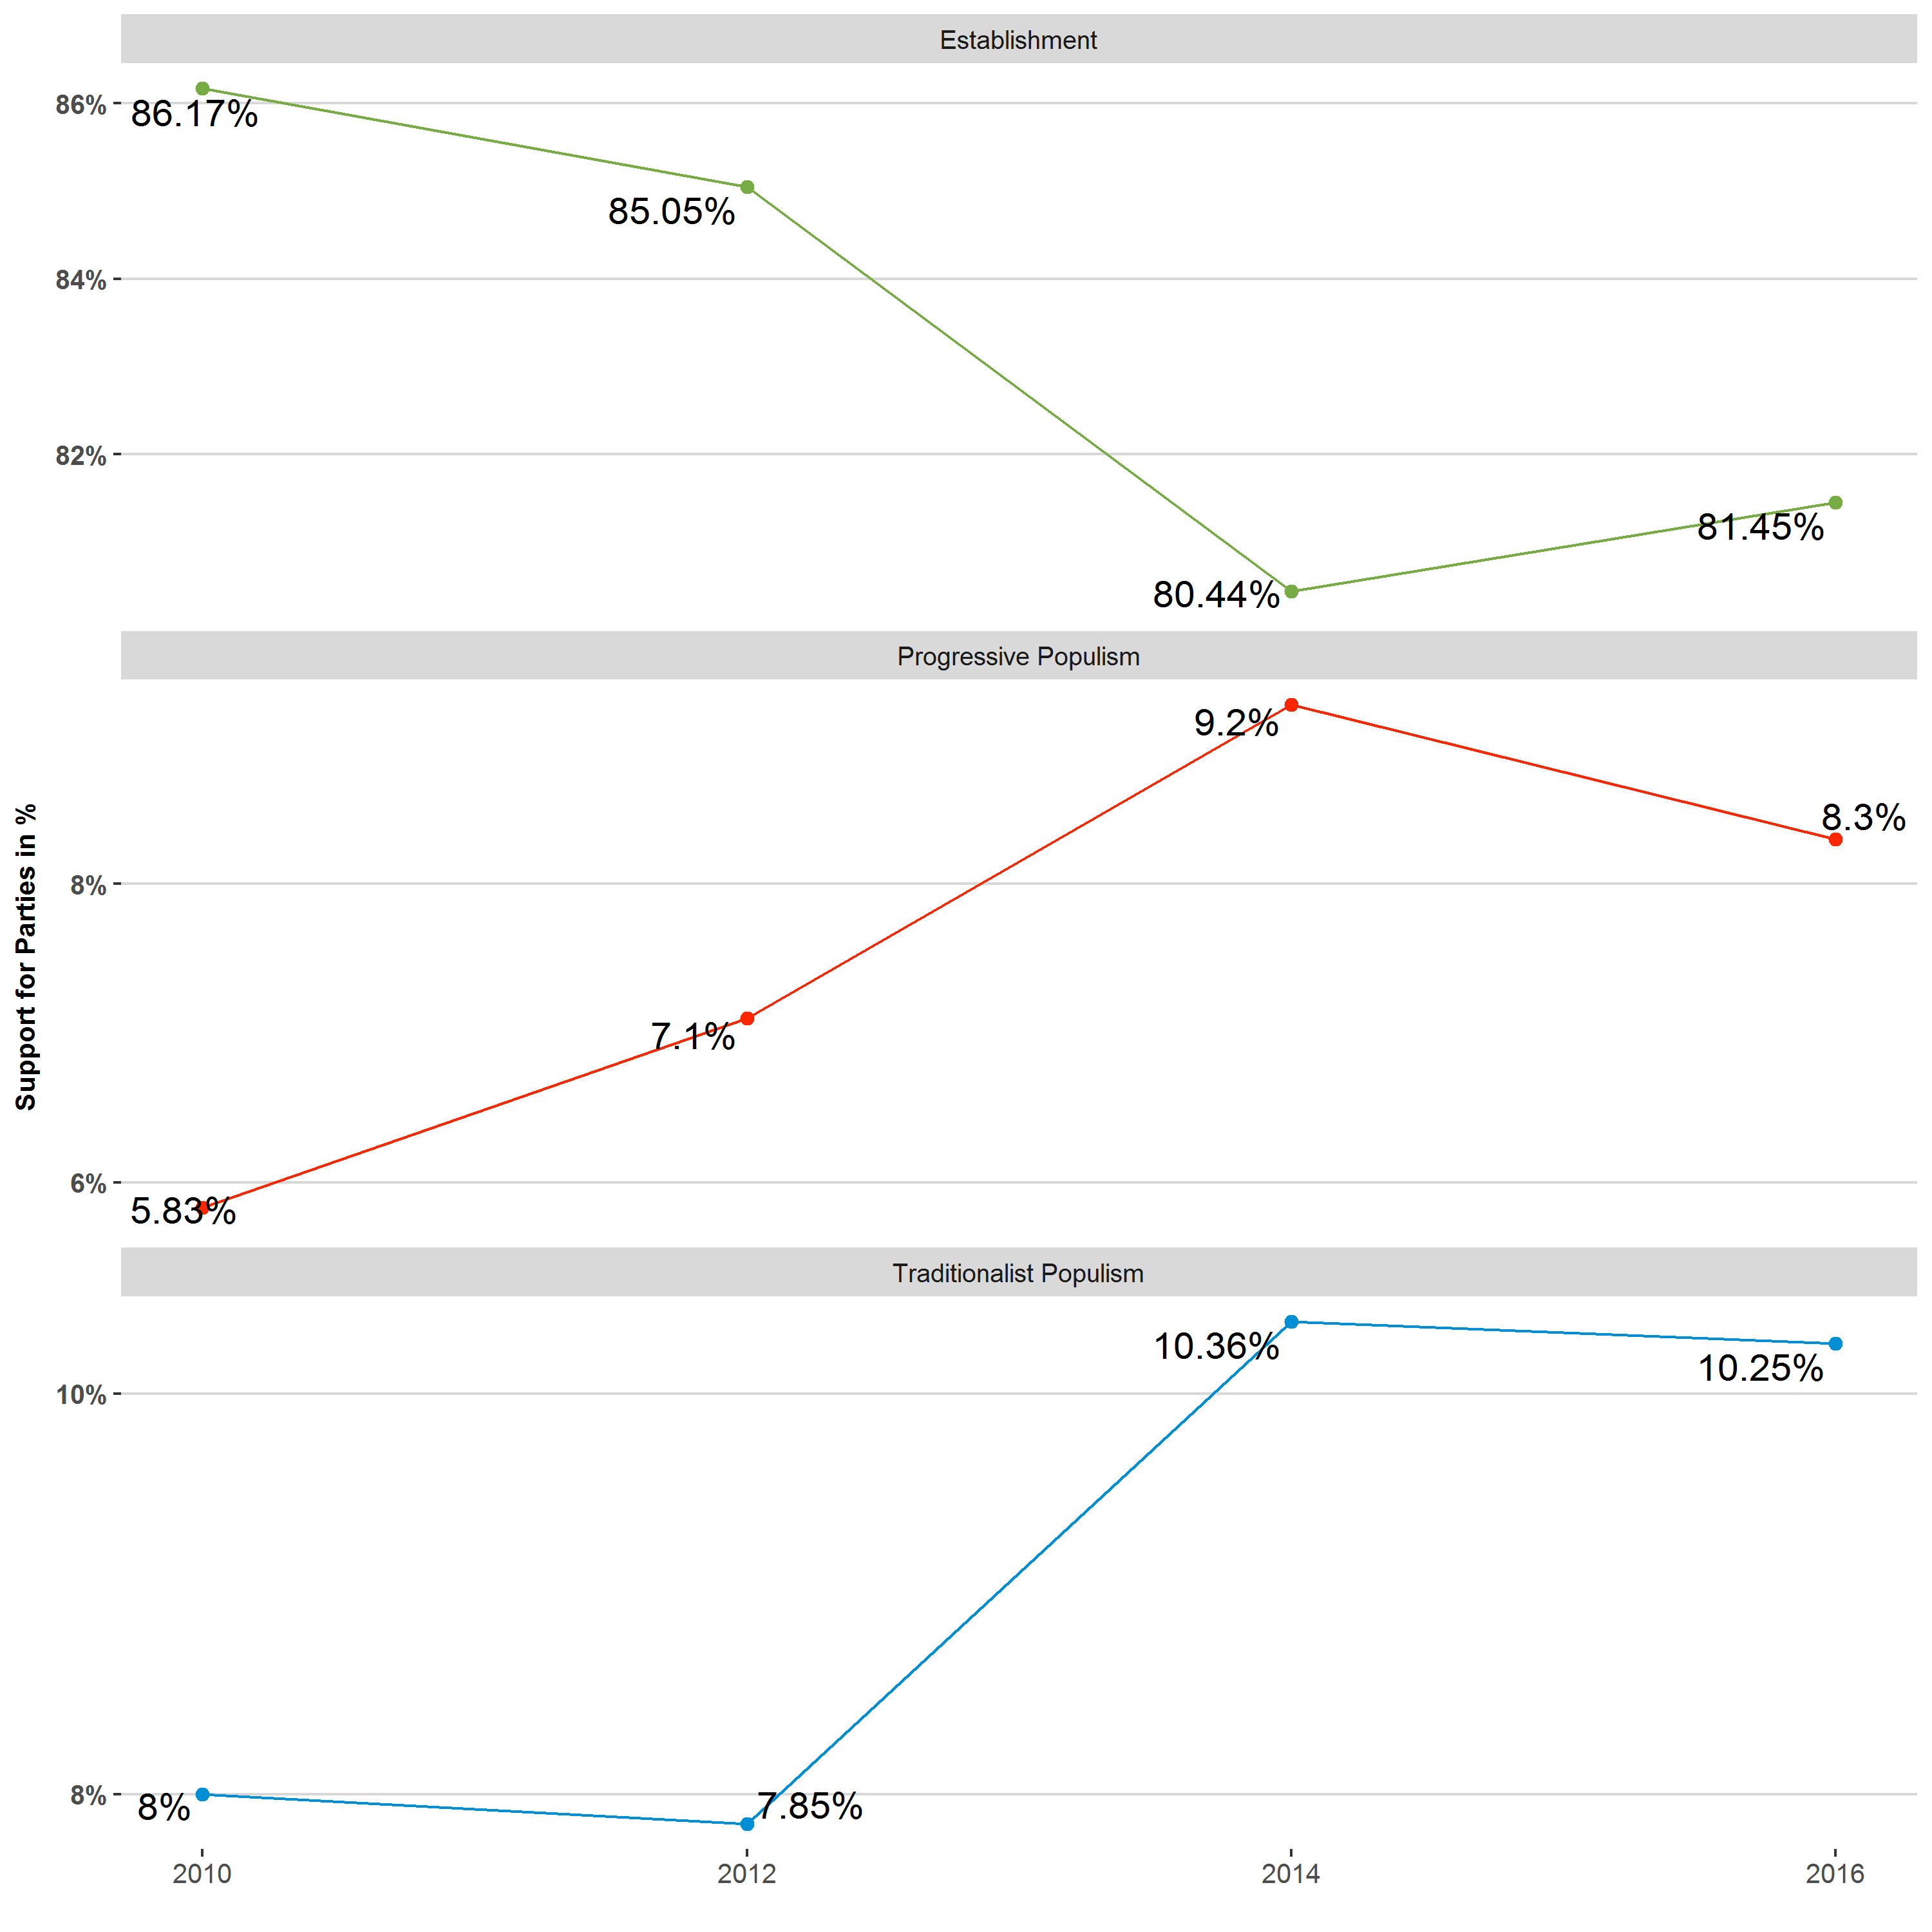
\includegraphics[width=\textwidth]{images/yearplot.png}
    \flushright
    {\scriptsize Source: ESS Data Round 5 - 8; N = 87238. \par}
\end{figure}

Figure \ref{yearplot} shows the support for populist and establishment
parties over the timerange that is present in our dataset (2010 - 2016).
As can be observed in the figure, support for populist parties has
increased in recent years and support for the establishment has fallen.
Support for established parties has dropped from 86.17\% in 2010 to
81.45\% in 2016, reaching the lowest point in 2014 with 80.44\%. The
opposite trend can be observed for the support of populist parties:
support for progressive populists has risen from 5.83\% in 2010 to 8.3\%
in 2016. In regards to traditionalist populism, there was an increase
from 8\% in 2010 to 10.25\% support in 2016. Support for progressive and
traditionalist populist parties peaked with 9.2\% and 10.36\%
respectively in 2014 and has remained relatively constant for 2016.

\begin{figure}[]
    \caption{Support for Establishment/Populist Parties Across European Regions}
    \label{regionplot}
    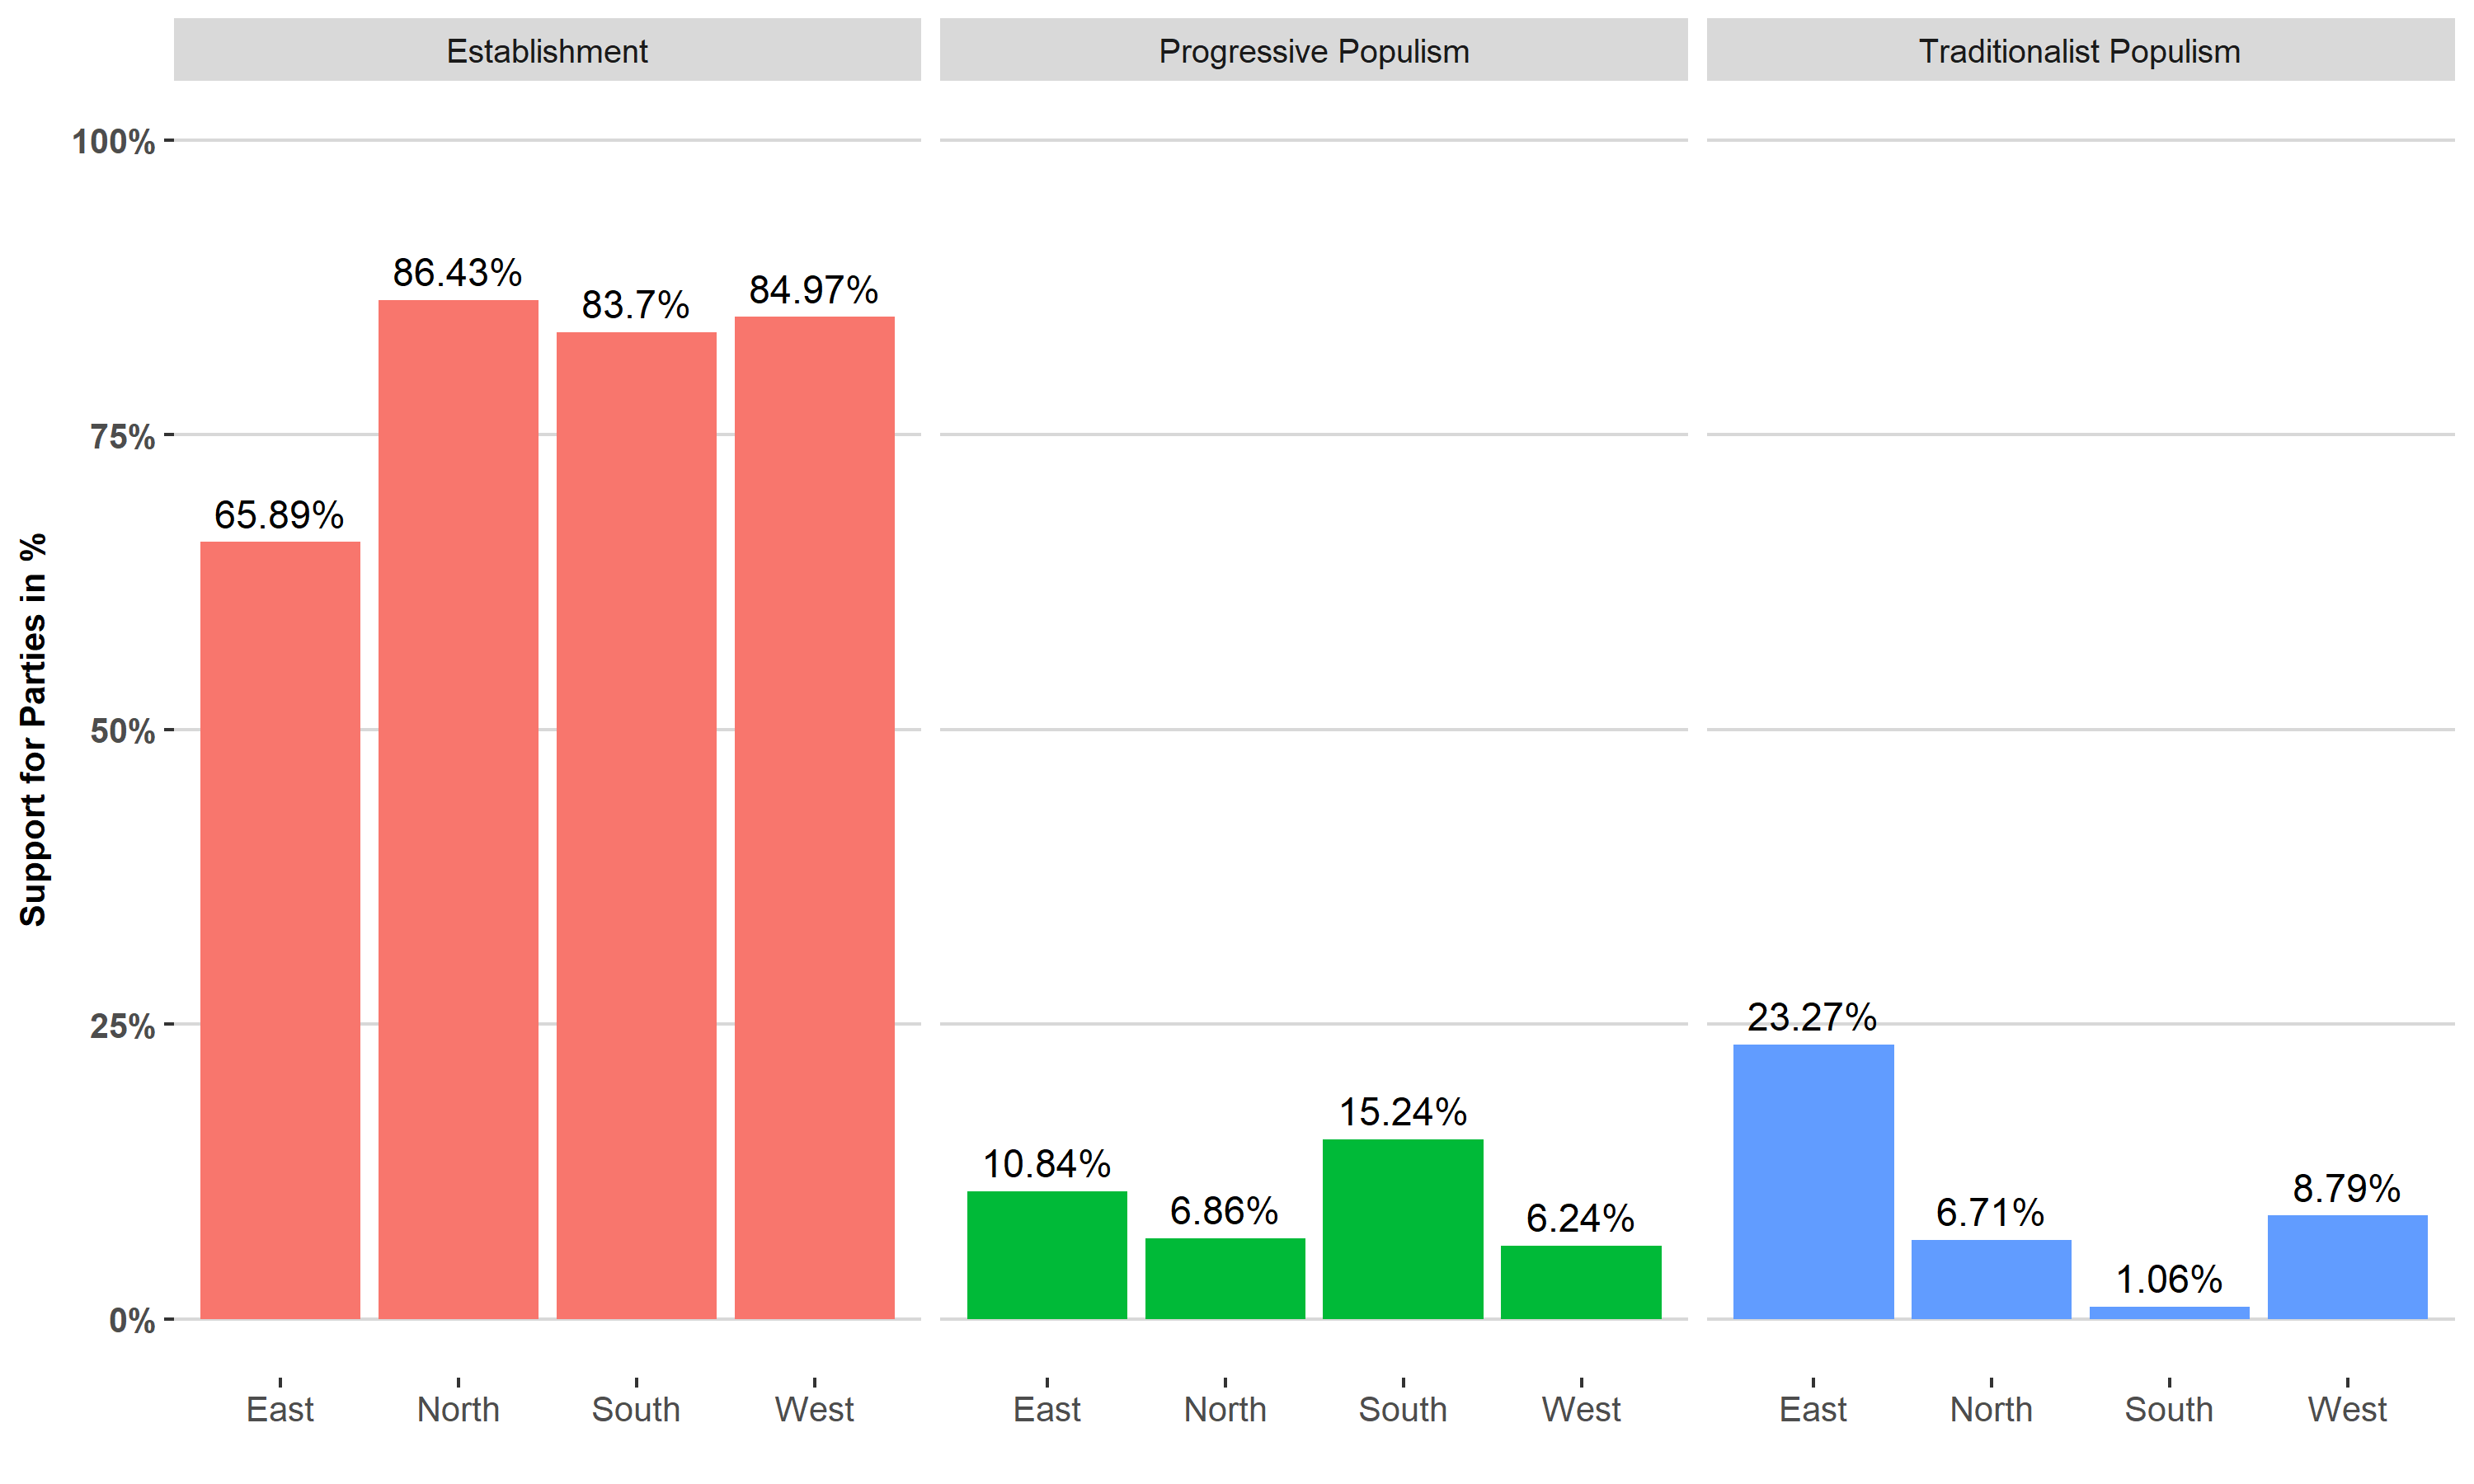
\includegraphics[width=\textwidth]{images/regionalplot.png}
    \flushright
    {\scriptsize Source: ESS Data Round 5 - 8; N = 87238. \par}
\end{figure}

Figure \ref{regionplot} visualizes the support of populist parties for
European regions as defined by the UN\footnote{Standard country or area
  codes for statistical use (M49). See:
  \url{https://unstats.un.org/unsd/methodology/m49/}}. It can be
observed that Eastern Europe stands out in regard to the support for
established parties, where it is significantly lower than in other
regions: only 65.89\% support established parties in Eastern Europe,
whereas in any other region support is well above 80\%. Most notably,
the support for non-establishment parties in Eastern Europe is primarily
due to traditional populists (23.27\%). Regarding the support of
progressive populists, the East does not stands out clearly anymore.

Southern Europe, like Northern and Western Europe, shows more than 80\%
support for established parties, but the south clearly stands out in
regard to their support for progressive populists (15.24\%). In regard
to traditionalist populists, a very different picture emerges for
Southern Europe, where support is just over 1\% and thus hardly worth
mentioning. Such low support for populists cannot be observed in any
other region, where the mininum is at least 6\%.

\textbf{potentielle Begr??ndungen k??nnen in dem zusammenfassenden
Absatz des Kapitels???oder man k??nnte auch weitere Plots machen, aber
muss ja ned sein}

\begin{figure}[!h]
    \caption{Support for Establishment/Populist Parties over Time}
    \label{plot2by2}
    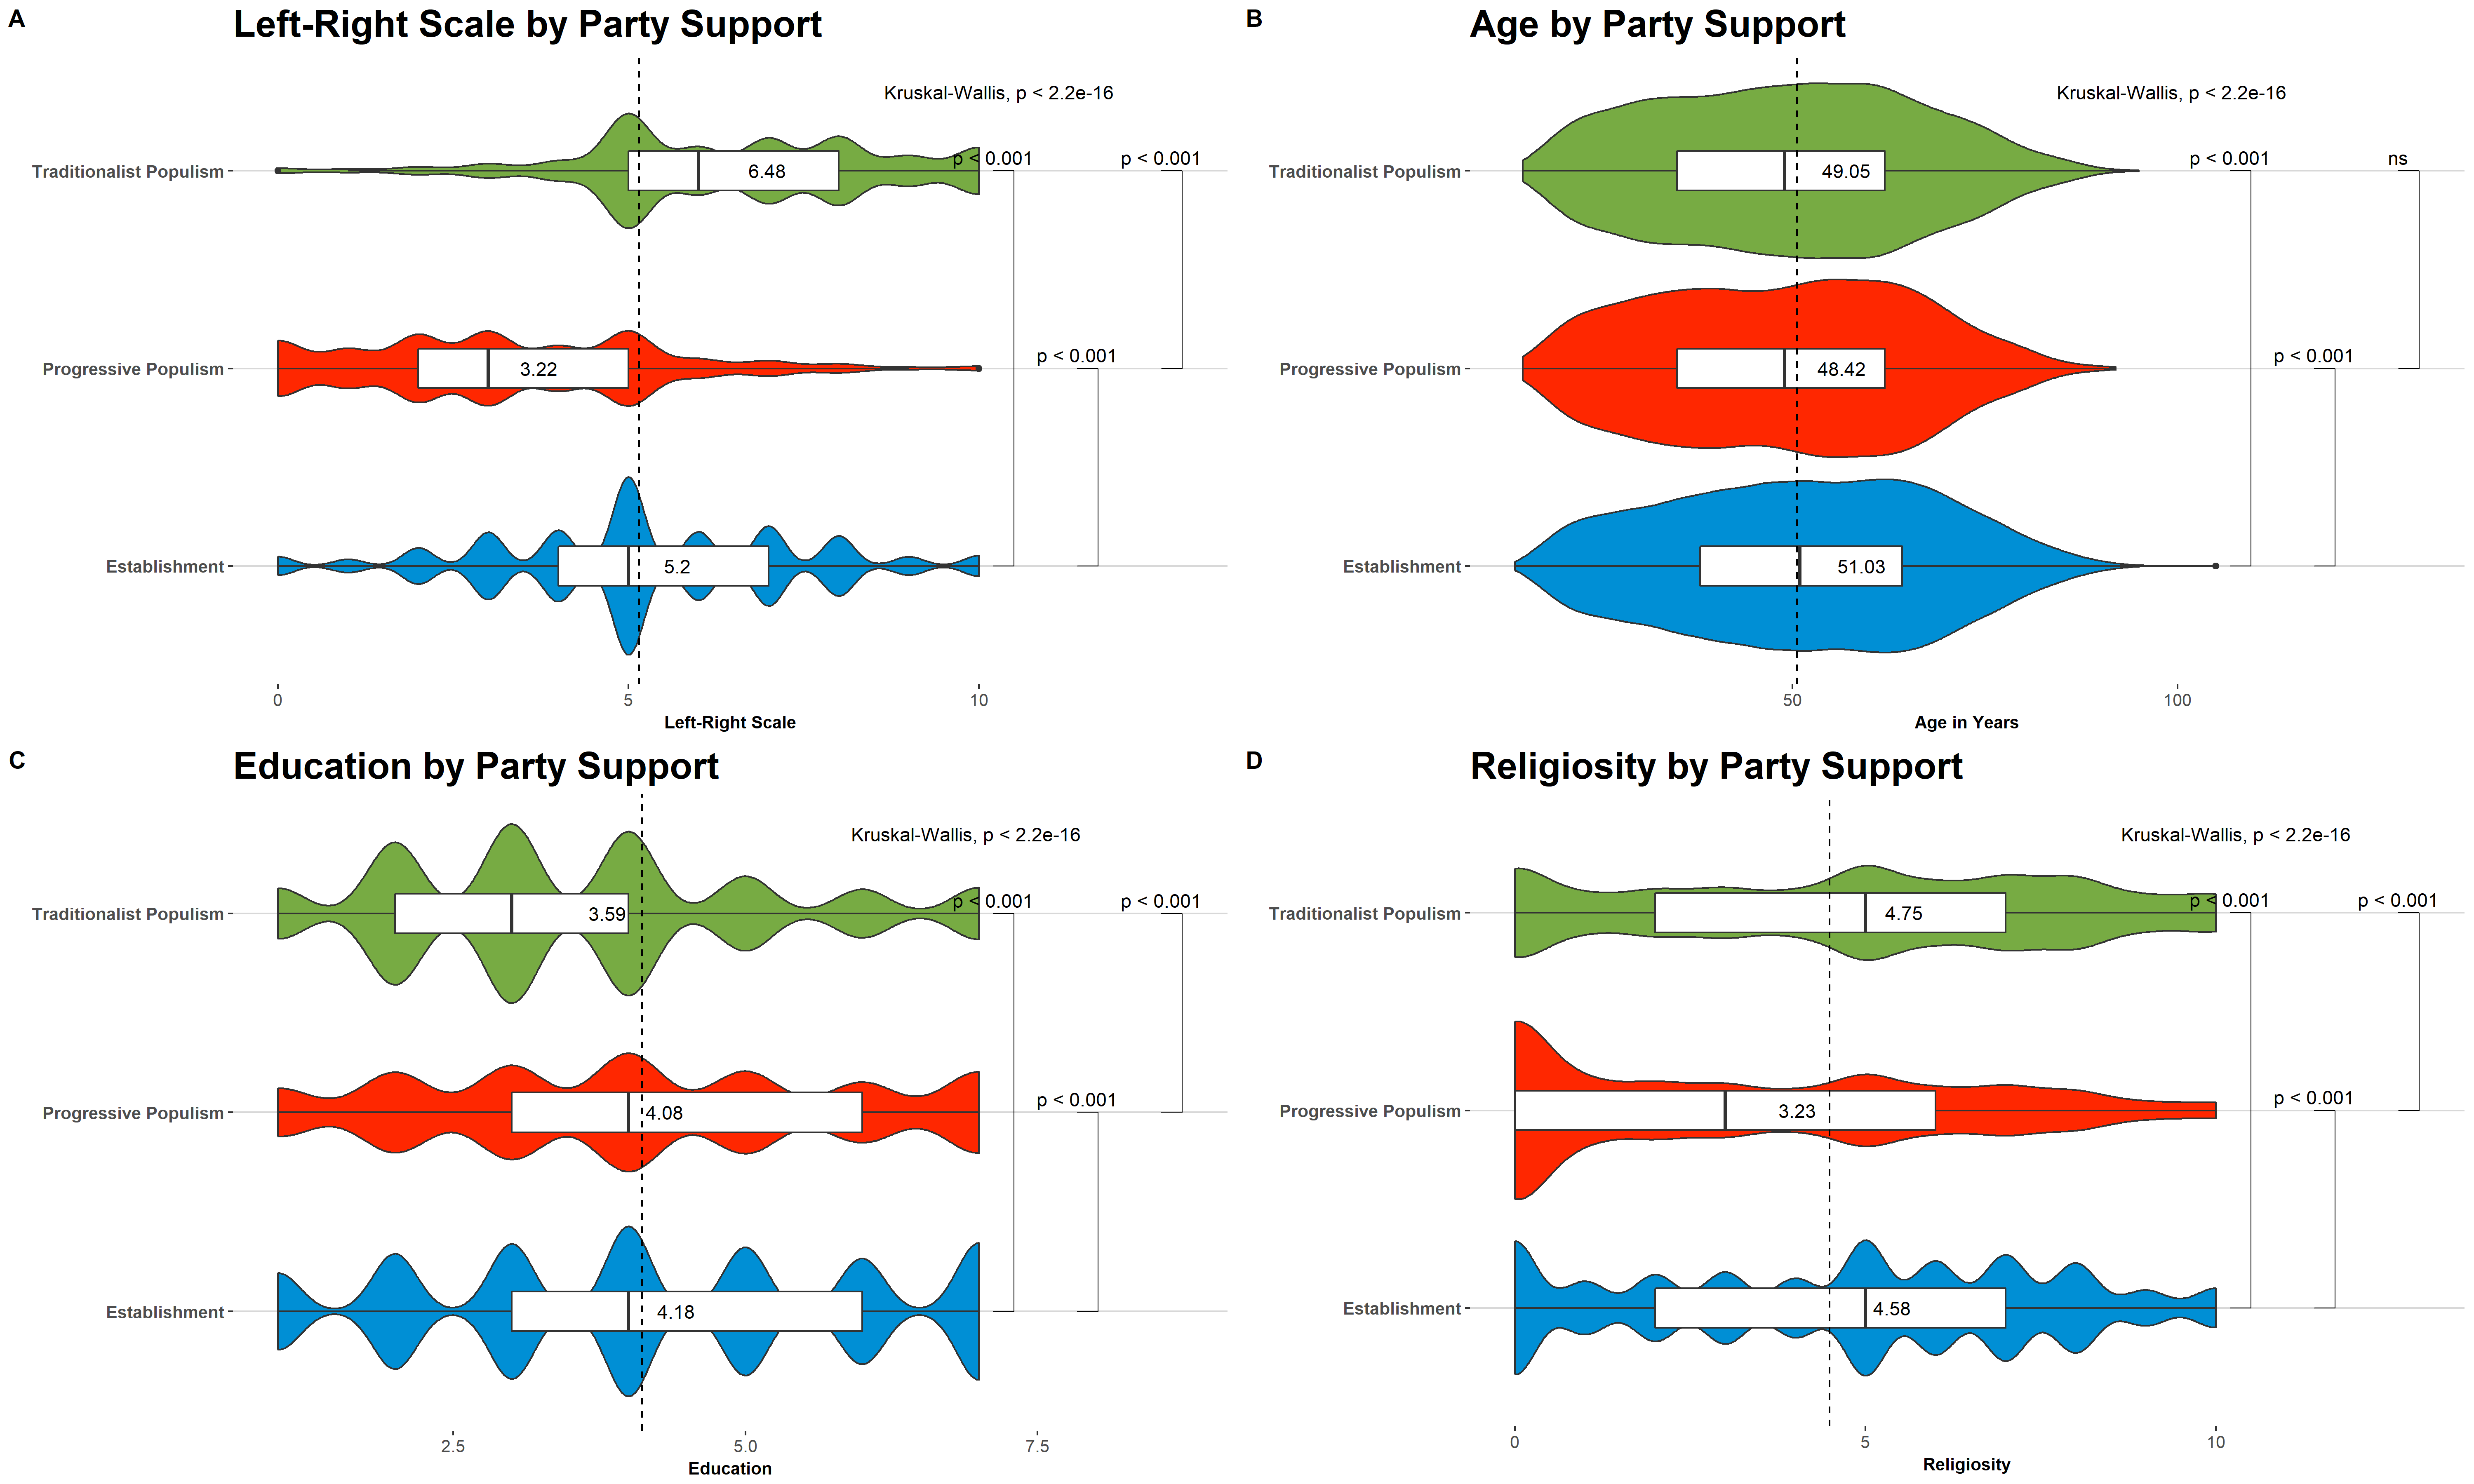
\includegraphics[width=\textwidth]{images/plot2by2.png}
    \flushright
    {\scriptsize Source: ESS Data Round 5 - 8; N = 87238. \par}
\end{figure}

With regard to socio-demographic characteristics, there are equally
clear trends. With regard to age, it becomes clear that supporters for
established parties are older than those who support populist parties.
Also, the differences between the group of supporters for established
parties over the other two groups are significant. There is no
significant difference between the groups ``supporters for traditional
populists'' and ``supporters for progressive populists'' regarding age.
In education, supporters for traditional populists stand out. These have
a much lower education than the supporters of established parties or
progressive populists. Although there are no visually identifiable
differences between supporters of progressive populists and supporters
of established parties, but an averaging comparison is significant. In
terms of religiousness, especially the supporters of the progressive
populists stand out with a lower average level of religiosity.
Supporters of traditional and established parties both share similar
religiosity, but, as mentioned on education before, a significant
difference between the two groups can be identified by comparing the
mean. A clear picture emerges regarding self-placement on the left-right
scale. Those who support progressive populists arrange themselves on
average in the left spectrum. On the other hand, the supporters of
traditional populists tend to be more in line with the right-wing
spectrum. In the case of the supporters for established parties, on
average there is a classification in the middle of the left-right
spectrum. Of course, this is more of a trivial finding, but these
results once again confirm our operationalization. \textbf{IMPORTANT:
mean einbauen, entweder in den Text oder aber in den Plot???damit sich
die Signifikanzen f??r den Leser noch mal besser erkl??ren //
statistische Kennwerte in den Text einbauen =\textgreater{} t-Werte..}

\subsection{logistic Analysis}\label{logistic-analysis}

This section will present the results of multinomial logistic regression
used to estimate the support for progressive and traditionalist
populism.

\subsection{Results}\label{results}

control: The results found in the descriptive part are confirmed in the
control model. In terms of age, the chance of support for both
progressive and traditional populists of higher age is 1.01 lower than
for support of established parties. In education, it is once again clear
that supporters of traditional populists have a significantly lower
education. Thus, the chance to support traditional populists compared to
support of established parties per education point is 1.28 lower, OR =
0.78; 95\% CI (0.77-0.79); p \textless{} 0.001. Even with respect to the
left-right spectrum, the previously descriptive identified
characteristics can be found clearly: the opportunity for support of
progressive populists compared to support for established parties is
lower by 1.45, whereas the chance for support of progressive populists
by 1.43 higher, OR = 0.69; 95\% CI (0.68-0.70); p \textless{} 0.001 and
OR = 1.43; 95\% CI (1.41-1.45); p \textless{} 0.001.

model1: First, the economic hypothesis will be examined. Here it can be
seen that the chance for support of progressive populists compared to
support of established parties increases by 1.20 per scale point in the
economic insecurity. Similarly, support for traditional populists is
similar. Here is the chance of this 1.34 higher. Similar effects can be
observed in unemployment, OR = 1.19; 95\% CI (1.11-1.26); p \textless{}
0.001 and OR = 1.34; 95\% CI (1.26-1.42); p \textless{} 0.001. With
regard to welfare, another picture is emerging. While there is a greater
chance for progressive populists to support 1.26 compared to support
from established parties, it should be noted that the effect is only
slightly significant. However, this does not seem to have any
significant effect on the support of traditional populists, OR = 0.94;
95\% CI (0.81-1.09); p = 0.40. In terms of the economic dimension, it
can be seen that as economic deprivation increases, the chance of
support for populists is higher compared to support from established
parties. However, the dependency on social benefits/welfare varies. In
addition, almost all effects are significant in the model, and
McFadden's R?? increases from 0.2 to 0.21 in Model 1 compared to the
control model. In addition, the fit of the model is significantly better
than the control model.

model2: Now we come to the cultural thesis. It clearly shows that anti
immigration has increased the chance for support from traditional
populists by 1.29 compared to support from established parties, OR =
1.29; 95\% CI (1.27-1.31); p \textless{} 0.001. There are also
differences regarding conservative attitudes. Thus, the chance of
supporting traditional populists is slightly higher compared to support
from established parties, whereas the chance of supporting progressive
populists is slightly lower. A similar difference can also be noted in
terms of openness. The effects on the self-enhancement scale and the
self-transcendence scale are in line with expectations. For each scale
point on the self-transcendence scale, the chance of support for
traditional populists is 1.08 lower than that for established party
support. Regarding the support for progressive populists, the chance are
slightly larger. With regard to the self-enhancement scale, the exact
opposite is the case with similar effect sizes. Not surprising are the
effects on government satisfaction and globalization. Globalization,
which has been measured by trust in the EU and the UN, as well as
satisfaction with the government, in comparison to the chance to support
established parties, less chance of supporting populist parties, OR =
0.92; 95\% CI (0.91-0.94); p \textless{} 0.001; OR = 0.93; 95\% CI
(0.92-0.95); p \textless{} 0.001; OR = 0.89; 95\% CI (0.88-0.91); p
\textless{} 0.001; OR = 0.88; 95\% CI (0.86-0.89); p \textless{} 0.001.
The McFadden's R?? increases from 0.21 to 0.24 compared to model 2, and
the fit of the model is significantly better compared to model 2. In
contrast to the economic dimension, the effects on the cultural
dimension went in different directions. It has thus become clear that
the cultural dimension ultimately contributes explanatory power when it
comes to the question of which form of populism is supported. However,
it should also be emphasized that the effect sizes found here are rather
weak.

Model 3: Model 3 now includes the economic as well as the cultural
dimensions. This confirms the previously found effects again. In terms
of the economic dimension, however, there are slight reductions in the
effects. But despite a slight weakening of the effect sizes,
significances remain untouched. Moreover, the McFadden's R?? increases
from 0.24 to 0.25 compared to model 2 and the fit of the model is
significantly better compared to the previous model.

Abschluss: Finally, with regard to our multinomial models, it can be
said that our hypotheses were able to confirm. Let's start with the
economic hypothesis:

H1: The less economically fortunate (economic dissatisfaction,
unemployment, economic insecurity, living on welfare), the higher the
probability of supporting anti-establishment parties.

This hypothesis was clearly confirmed by the models. Unemployment,
economic insecurity and also the life on welfare increase the chance to
support populists compared to support of established parties. The impact
of living on welfare seems not to be as great as the other two factors
mentioned and does not even have a significant effect in supporting
traditional populists. In addition, in Model 3, where the cultural
dimension has been added, there is a slight weakening of the effects.
But despite the weakening, all significances remain stable.

Concerning our two established culture hypotheses, confirmatory results
could also be found here. H2: The more culturally inclusive (values),
the higher the probability of supporting progressive populist parties.

H3: The more culturally exclusive, the higher the probability of
supporting a traditionalist populist party.

Inclusive values (high values for self-transcendence and openness and a
low value for anti-immigration) increases the probability of support for
progressive populists, but openness has no significant effect here.
Also, when there are exclusive values (low values for self-transcendence
and openness and a high value for anti-immigration), the probability of
supporting traditional populists increases. Anti-immigration in
particular seems very important here and stands out clearly from the
other effects. In addition, the effect of openness on supporting
traditional populist parties is highly significant. Even in Model 3, all
these effects remain stable. The effects also show our previously
suspected differentiation. The economic dimension generally provides for
an increase in the likelihood of supporting populist parties. The
cultural dimension, on the other hand, shows that it has an opposite
effect on the support of traditional and progressive populists.

It should also be stressed that while all the effects found are
significant, they are rather weak. In addition, almost all effects of
the control variables remain significant in all models. In literature,
supporters of populist parties often associate features such as a higher
age and lower education. But there were slight surprises here. The
strong difference between supporting progressive and traditional
populists in education stands out. Supporters of traditional populists
may have low education but not supporters of progressive populists. When
it comes to age, it even shows that supporters of progressive populists
as well as supporters of traditional populists have a slightly lower
age.

Let's first evaluate the results of the \emph{economic deprivation
hypothesis}. Looking at \emph{Welfare}, the chance of supporting a
traditionalist populist party compared to supporting an Establishment
party seems to not have a significant effect, OR = 1.05; 95\% CI
(0.90-1.23); p = 0.53. However, the expected effect of welfare emerges
elsewhere: the chance of supporting a progressive party compared to an
establishment party is 1.29 higher when an individual is on welfare, OR
= 1.29; 95\% CI (1.14-1.47); p \textless{} 0.001.

Let's next evaulate the effects for the \emph{cultural thesis}. Looking
at \emph{Conservation}, the chance of supporting a traditionalist
populist party compared to supporting an Establishment party seems to
increase by 1.05 per conservation unit scale, OR = 1.05; 95\% CI
(1.03-1.08); p \textless{} 0.001. The expected effect of
\emph{Conservation} also emerges when looking at progressive populism:
the chance of supporting a progressive party compared to an
establishment party is 1.03 lower when an individual fully endorses
conservation values, OR = 0.97; 95\% CI (0.95-1.00); p \textless{} 0.05.

\begin{landscape}
\begin{figure}[htpb]
  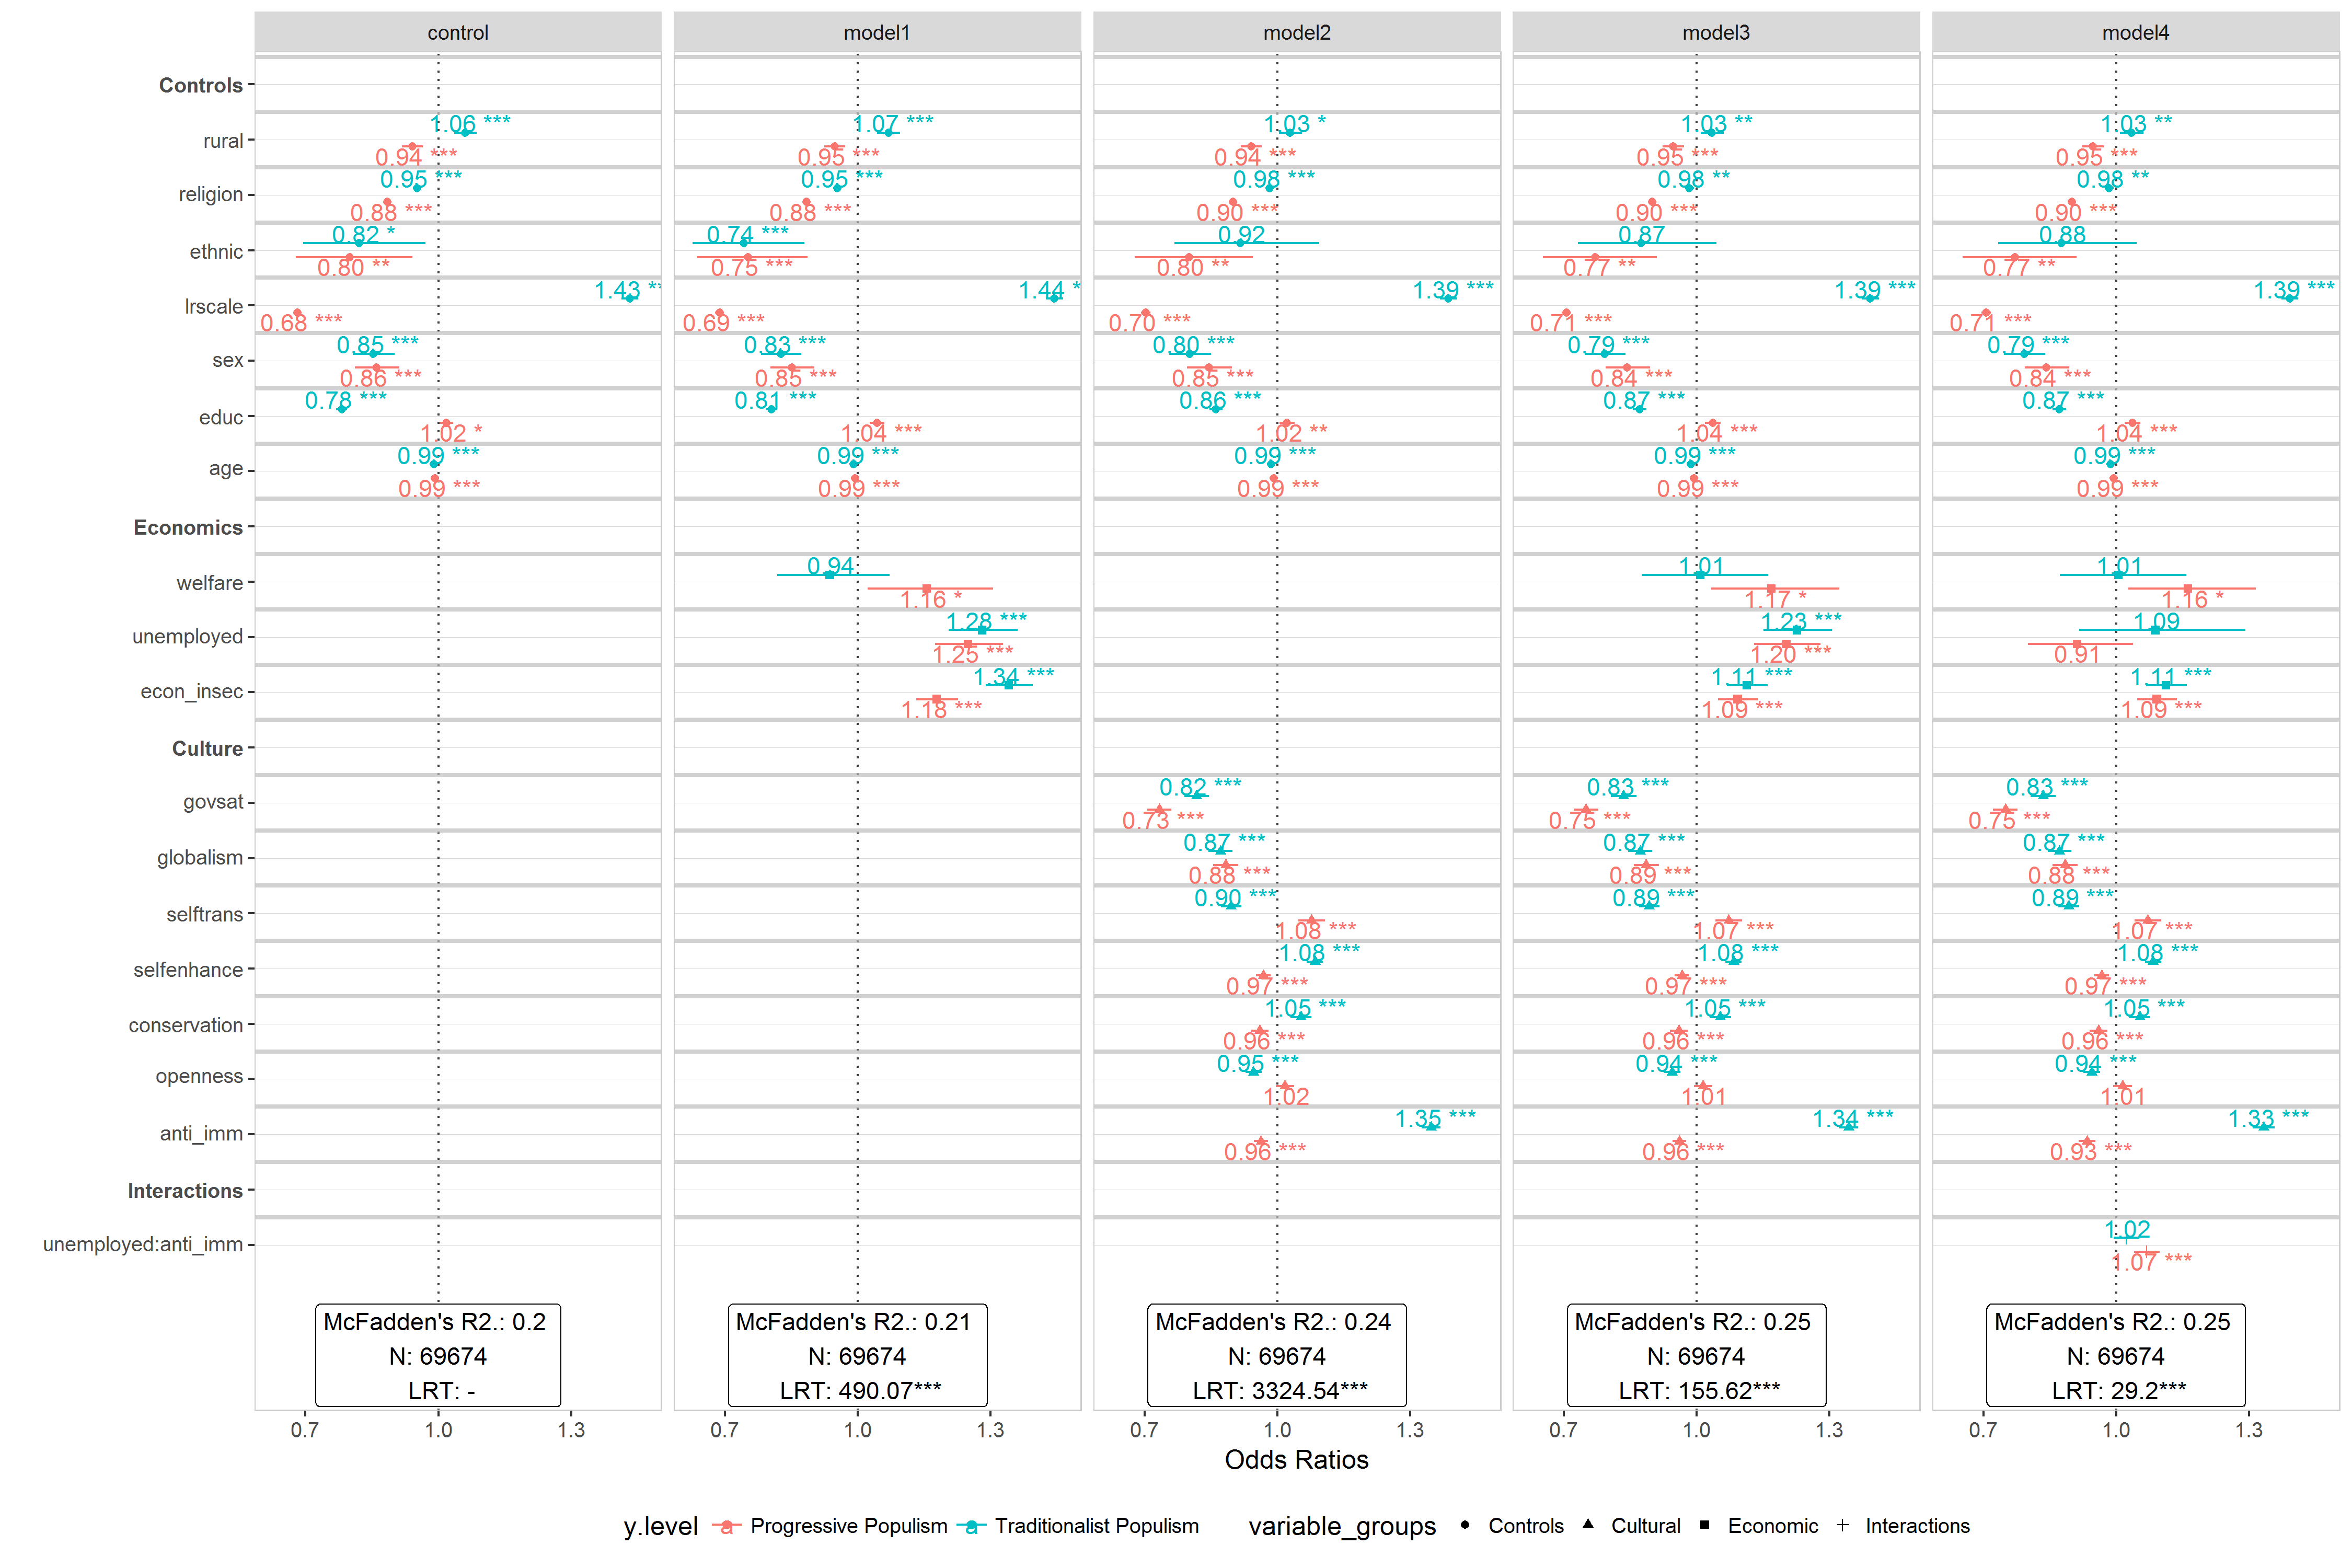
\includegraphics[height=1.2\textheight, width=1.5\textwidth]{images/onebigmotherfucker.png}
  \caption{Functional Decomposed Data Structure}
\end{figure}
\end{landscape}


\end{document}
